%%%%%%%% ICML 2026 WORKSHOP SUBMISSION %%%%%%%%%%%%%%%%
%
% Anonymous submission. Compile:
%   pdflatex paper && bibtex paper && pdflatex paper && pdflatex paper

\documentclass{article}

\usepackage{microtype}
\usepackage{graphicx}
\usepackage{subcaption}
\usepackage{booktabs}
\usepackage{multirow}
\usepackage{array}
\usepackage{hyperref}
\usepackage{tikz}
\usetikzlibrary{arrows.meta,positioning,fit,calc}

\newcommand{\theHalgorithm}{\arabic{algorithm}}

\usepackage{icml2026}

\usepackage{amsmath}
\usepackage{amssymb}
\usepackage{mathtools}
\usepackage{amsthm}
\usepackage[capitalize,noabbrev]{cleveref}

\theoremstyle{plain}
\newtheorem{theorem}{Theorem}[section]
\newtheorem{proposition}[theorem]{Proposition}
\theoremstyle{definition}
\newtheorem{definition}[theorem]{Definition}

\newcommand{\ours}{\textsc{MultiPass}}
\newcommand{\dkmp}{\textsc{DKMP}}
\newcommand{\lm}{\textsc{LongMemEval}}

\icmltitlerunning{Bridge Starvation: A Failure Mode of Single-Pass Memory Retrieval}

\begin{document}

\twocolumn[
  \icmltitle{\texorpdfstring{Bridge Starvation: A Reproducible Failure Mode of\\
    Single-Pass Memory Retrieval, with a Bounded Repair}{Bridge Starvation: A Reproducible Failure Mode of Single-Pass Memory Retrieval, with a Bounded Repair}}

  \icmlsetsymbol{equal}{*}

  \begin{icmlauthorlist}
    \icmlauthor{Anonymous Authors}{anon}
  \end{icmlauthorlist}

  \icmlaffiliation{anon}{Anonymous Institution}

  \icmlcorrespondingauthor{Anonymous Authors}{anonymous@anon.org}

  \icmlkeywords{agentic memory, multi-hop retrieval, failure modes,
    long-context reasoning, fault injection}

  \vskip 0.3in
]

\printAffiliationsAndNotice{}

\begin{abstract}
Long-horizon agents can fail long before their final answer: a missed
memory item at an early step quietly removes the evidence needed later.
We isolate a reproducible instance of this problem in single-pass
agentic-memory retrieval. The failure, which we call \emph{bridge
starvation}, occurs when a query names entity $X$ but the answer requires a
chain $X{\to}Y{\to}Z{\to}\dots$; the first retrieval pass finds the $X$
fact, but the bridge entities are absent from the query and the remaining
links are never retrieved. We introduce \dkmp{}, a controlled trigger that
varies chain depth (2--5 hops) and context length (1K--128K tokens), and
we pair it with trace diagnostics that separate retrieval coverage from
reader composition. As a bounded repair, \ours{} reuses the same retriever
but asks the LLM to emit one short bridge entity between retrieval passes.
On the targeted 2/3/4-hop, 128K-token regime, \ours{} reaches 1.00, 0.90,
and 0.97 accuracy ($n{=}30$ per cell), within 3pp of the gold-support
oracle on 3/4-hop and above IRCoT, ReAct, Self-Ask, and a passage-graph
PPR variant under the same reader and index. The repair has clear
boundaries: it does not solve 5-hop chains, where coverage falls to 0.75
and reader composition becomes a second failure mode; it does not help on
short-context MuSiQue, where the trigger does not fire; and it does not
target the cross-session aggregation failure that dominates \lm{}. We
release the trigger, traces, and per-pass diagnostics.
\end{abstract}

\begin{figure*}[t]
\centering
\resizebox{\textwidth}{!}{%
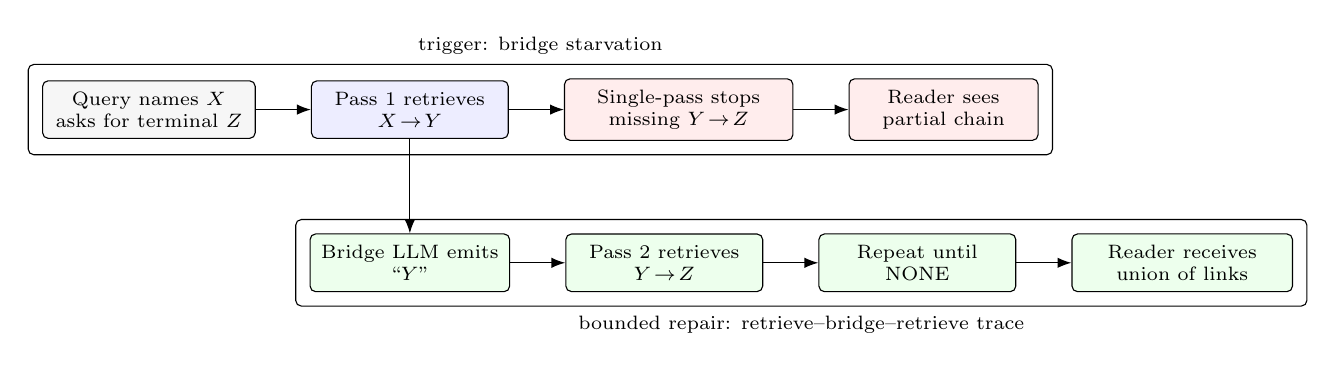
\begin{tikzpicture}[
  font=\scriptsize,
  >=Latex,
  box/.style={draw, rounded corners=2pt, align=center, minimum height=7mm,
    inner sep=4pt, fill=gray!7},
  hit/.style={draw, rounded corners=2pt, align=center, minimum height=7mm,
    inner sep=4pt, fill=blue!7},
  miss/.style={draw, rounded corners=2pt, align=center, minimum height=7mm,
    inner sep=4pt, fill=red!7},
  fix/.style={draw, rounded corners=2pt, align=center, minimum height=7mm,
    inner sep=4pt, fill=green!7},
  arrow/.style={->, line width=0.45pt}
]
  \node[box, minimum width=27mm] (q) {Query names $X$\\asks for terminal $Z$};
  \node[hit, minimum width=25mm, right=7mm of q] (xy) {Pass 1 retrieves\\$X\!\to\!Y$};
  \node[miss, minimum width=29mm, right=7mm of xy] (miss) {Single-pass stops\\missing $Y\!\to\!Z$};
  \node[miss, minimum width=24mm, right=7mm of miss] (wrong) {Reader sees\\partial chain};

  \node[fix, minimum width=25mm, below=12mm of xy] (bridge1) {Bridge LLM emits\\``$Y$''};
  \node[fix, minimum width=25mm, right=7mm of bridge1] (yz) {Pass 2 retrieves\\$Y\!\to\!Z$};
  \node[fix, minimum width=25mm, right=7mm of yz] (bridge2) {Repeat until\\NONE};
  \node[fix, minimum width=28mm, right=7mm of bridge2] (reader) {Reader receives\\union of links};

  \draw[arrow] (q) -- (xy);
  \draw[arrow] (xy) -- (miss);
  \draw[arrow] (miss) -- (wrong);
  \draw[arrow] (xy) -- (bridge1);
  \draw[arrow] (bridge1) -- (yz);
  \draw[arrow] (yz) -- (bridge2);
  \draw[arrow] (bridge2) -- (reader);

  \node[draw, rounded corners=2pt, fit=(q)(xy)(miss)(wrong), inner sep=5pt,
    label={[font=\scriptsize]above:trigger: bridge starvation}] {};
  \node[draw, rounded corners=2pt, fit=(bridge1)(yz)(bridge2)(reader), inner sep=5pt,
    label={[font=\scriptsize]below:bounded repair: retrieve--bridge--retrieve trace}] {};
\end{tikzpicture}
}
\caption{Bridge starvation and the \ours{} repair. Single-pass retrieval
matches the query entity $X$ and retrieves the first link, but bridge
entities are absent from the query and therefore starve subsequent passes.
\ours{} turns the failure into an observable trace: the LLM emits one short
bridge entity, the same retriever is called again, and chain coverage can be
measured after each pass.}
\label{fig:mechanism}
\end{figure*}

% =============================================================================
\section{Introduction}\label{sec:intro}

A foundation-model agent often acts through a memory layer: it reads a
long trace of prior turns, retrieves a few relevant items, and conditions
the next step on those items. Reliability failures at this layer are hard
to diagnose because the visible error may occur long after the missing
memory item. A wrong final answer can therefore hide a simpler upstream
question: did the agent ever retrieve the evidence needed to answer?

This paper isolates one retrieval-layer failure that is small enough to
reproduce and sharp enough to repair. Many proposed agentic-memory systems
expose a single-pass retrieval interface at inference: given the current
query or state, retrieve a small set of memory items and pass them to a
reader. The extraction, storage, and consolidation pipelines around this
interface differ substantially. Examples where the single-pass interface
is visible include Mem0~\cite{mem0blog2026},
MemoryOS~\cite{memoryos2025emnlp}, and A-Mem~\cite{xu2025amem}; our claim
is about this interface, not about every component of these systems.

The failure appears when the query names the first entity in a chain but
not the later bridge entities. A question may ask for an attribute of the
city where $X$'s purchase was originally cut. The first retrieval pass can
find the sentence linking $X$ to the purchase, but the city name is not in
the query until that first sentence is read. A single-pass retriever
therefore has no opportunity to search for the next link. We call this
failure \emph{bridge starvation}. \Cref{fig:mechanism} shows the trace:
retrieval stops after the first link, while the repair exposes the missing
bridge entity and retrieves again.

To make the failure reproducible, \dkmp{} varies chain depth
$D \in \{2,3,4,5\}$ and context length
$N \in \{1K,8K,32K,128K\}$ over 30 stories per cell. Synthetic chain
entities prevent the reader from answering by prior knowledge. At
$N{=}128$K, single-pass hybrid retrieval scores 0.40 / 0.47 / 0.57 / 0.13
on 2/3/4/5-hop chains, against a gold-support oracle of
1.00 / 0.93 / 1.00 / 0.76 (\Cref{tab:main}).

\ours{} repairs the specific retrieval failure without changing the
retrieval index. Between passes, the LLM emits one short noun phrase
($\le 6$ words) naming the next entity to look up; the retriever runs
again with that phrase; and the final reader receives the union of
retrieved chunks. The loop stops adaptively when the bridge call emits
NONE. On the targeted 2/3/4-hop regime, \ours{} approaches oracle accuracy
with 4--5 LLM calls per query and outperforms four iterative-retrieval
baselines under the same reader.

The repair is intentionally bounded. It does not solve 5-hop chains: chain
coverage drops to 0.75 and the reader must also compose more facts. It
does not improve short-context MuSiQue, where the trigger does not fire.
It also does not target \lm{}'s dominant cross-session aggregation
failure, where there is no obvious next entity to retrieve.

Our contributions are:
\begin{itemize}\setlength{\itemsep}{0.05em}
  \item We define single-pass bridge starvation as an operational failure
        with explicit trigger and non-trigger conditions.
  \item We introduce \dkmp{}, a controlled trigger that measures the
        failure across chain depth and context length.
  \item We provide trace diagnostics that separate retrieval coverage from
        reader composition.
  \item We evaluate a bounded repair with measured cost and report the
        cases where the repair does not apply.
\end{itemize}

% =============================================================================
\section{Related Work}\label{sec:related}

Several retrieval-time reasoning methods already revisit the corpus
during generation, but they do not isolate bridge starvation as a failure
mode. IRCoT~\cite{trivedi2023ircot} interleaves retrieval with one
chain-of-thought sentence per step, originally using eight in-context
demonstrations and a \texttt{remove\_wh\_words} BM25 reformulation.
ReAct~\cite{yao2023react} alternates Thought / Action$_\text{Search}$ /
Observation, Self-Ask~\cite{press2023selfask} decomposes the question into
follow-ups, FLARE~\cite{jiang2023flare} triggers retrieval on uncertainty,
and HippoRAG~\cite{gutierrez2024hipporag} runs personalized PageRank over
an OpenIE-derived passage graph. We re-implement IRCoT in both 0-shot and
faithful 8-shot variants, plus ReAct, Self-Ask, and a passage-graph PPR
variant of HippoRAG without OpenIE. All baselines share the same reader and
retrieval index as \ours{}.

Agentic-memory systems differ in how they write and organize memory, so
same-reader comparisons are important when evaluating the retrieval layer.
Mem0~\cite{mem0blog2026} extracts atomic facts and stores them in a vector
store. MemoryOS~\cite{memoryos2025emnlp} adds hierarchical
operating-system layers. A-Mem~\cite{xu2025amem} introduces note-link
expansion at retrieval. We implement \emph{Mem0-style} memory
(LLM-extracted facts + cosine retrieval) and \emph{A-Mem-style} retrieval
(top-$K$ + 1-hop note-link expansion) under the same GLM-4.7 reader as our
chunk baseline (\Cref{tab:longmemeval}).

Long-context and multi-hop benchmarks provide useful controls but stress
different mechanisms. Lost-in-the-middle~\cite{liu2024lostmiddle} predicts
that full-context readers degrade when relevant content appears mid-input;
\dkmp{} length curves quantify this effect for our reader. MuSiQue
~\cite{musique} is a natural multi-hop QA benchmark with short contexts,
so we use it as a non-trigger control (\Cref{sec:musique}). \lm{}
~\cite{wu2024longmemeval} is a long-term-memory benchmark whose dominant
failure type is cross-session aggregation (\Cref{sec:longmemeval}).

% =============================================================================
\section{Operational Failure and \dkmp{} Trigger}\label{sec:dkmp}

\begin{definition}[Single-pass bridge starvation]
\label{def:bridge-starvation}
A query $q$ names entity $X$ and asks for a terminal answer reachable only
by traversing a chain $Y_0{=}X \to Y_1 \to \cdots \to Y_D{=}Z$.
A single-pass top-$K$ retriever scores chunks against $q$ and returns the
chunk containing $Y_0{\to}Y_1$. Subsequent bridge facts
($Y_i{\to}Y_{i+1}$ for $i\ge1$) are absent from $q$, so they are not
retrieved. The reader answers from an incomplete chain.

\smallskip
\textit{Triggering preconditions.}
(a) chain depth $D \ge 2$;
(b) context $N$ large enough that full-context reading degrades --- in our
setup, $N \gtrsim 8K$ tokens;
(c) bridge entities $Y_i$ are not lexically present in $q$;
(d) retrieval is performed in one pass.

\smallskip
\textit{Non-trigger boundaries.}
short contexts where the reader can read everything;
single-hop probes; aggregation-style questions with no bridge entity in $q$;
settings where the reader is given gold support directly.
\end{definition}

\dkmp{} is built from 30 NarrativeQA stories. For each
$(\text{story}, D)$ pair with $D \in \{2,3,4,5\}$, GLM-4.7 generates one
chain of $D$ needles using a directional prompt with synthetic entity names
(e.g., ``Vixenia Strode'', ``Velorum'') chosen to avoid lexical collision
with the source story. We validate each chain by entailment.

The contexts at $\{1K, 8K, 32K, 128K\}$ tokens are built by sampling
distractor passages from \emph{other} stories and inserting needle
sentences at separate non-edge positions. The full trigger has
4 depths $\times$ 4 lengths $\times$ 30 stories $=$ 480 contexts. We also
include five single-hop probe types (lexical, paraphrase, coreference,
temporal-order, and causal-direction) as sanity checks. These probes
saturate at oracle for any reasonable retriever (avg.\ 0.97), so we omit
them from the main analysis.

GLM-4.7 ($T{=}0$, \texttt{thinking=off}) reads the retrieved context and
answers in one short sentence. A separate fresh GLM-4.7 call judges YES/NO
against the gold reference, so all reported accuracies are LLM-judge
accuracies. Synthetic entities remove a world-knowledge shortcut: an entity
such as ``Crystal of Mar'' has no Wikipedia article, so the only path to
the answer is retrieval and chain traversal.

% =============================================================================
\section{Bounded Repair: \ours{}}\label{sec:method}

Given query $q$ and a chunked corpus, \ours{}:
\begin{enumerate}\setlength{\itemsep}{0.05em}
  \item Initialize $\mathcal{C}\gets\emptyset$, $q_0\gets q$.
  \item For $i \in \{0,\ldots,D_{\max}{-}1\}$:
    \begin{itemize}\setlength{\itemsep}{0.05em}
      \item Retrieve $\mathrm{top}_K(q_i)$, dedup against $\mathcal{C}$,
            append.
      \item Bridge prompt: ``Given $q$ and $\mathcal{C}$, name the next
            intermediate entity to look up ($\le 6$ words), or NONE if done.''
      \item Parse $b_i \gets \mathrm{LLM}$. If NONE or empty, break.
      \item $q_{i+1} \gets b_i$.
    \end{itemize}
  \item Final reader call: ``Answer $q$ using $\mathcal{C}$.''
\end{enumerate}

For a chain that stops adaptively after $D^\star \le D_{\max}$ passes,
\ours{} issues $D^\star$ retrievals, $D^\star$ short bridge LLM calls
(the last may emit NONE), and one final reader call, for $D^\star{+}1$
LLM calls in total. Each bridge call has output capped at 30 tokens. Only
the final reader sees the full retrieved context.

This design targets bridge starvation as defined in \Cref{sec:dkmp}. The
LLM names the next bridge entity, and the retriever locates the next link.
The method does \emph{not} directly solve reader composition, because the
reader still has to chain $D$ facts at the end. It also does not solve
aggregation queries when there is no obvious bridge entity to emit.

% =============================================================================
\section{Trace Diagnostics}\label{sec:trace}

We log every retrieval, every bridge-LLM call, and every reader call. The
trace exposes failure modes that final-answer accuracy hides.

\subsection{Schematic minimal trace}

Figure~\ref{fig:mechanism} shows the minimal trace. On a 3-hop chain
$X{\to}Y{\to}Z{\to}W$, single-pass retrieval stops after retrieving
$X{\to}Y$; \ours{} emits ``$Y$'', retrieves $Y{\to}Z$, emits ``$Z$'',
retrieves $Z{\to}W$, then stops with NONE. Appendix~\ref{appx:trace}
gives a real DKMP trace.

\subsection{Chain-coverage diagnostic}

For each $(D,\text{method})$ cell at $N{=}128$K we measure
ChainFactRecall = fraction of gold needle sentences that appear in any
retrieved chunk after the method finishes. \Cref{tab:coverage} gives the
breakdown.

\begin{table}[t]
\centering
\caption{Chain coverage and answer accuracy for \ours{} at $N{=}128$K
($n{=}30$/cell). For 2/3/4-hop, coverage is essentially complete and the
small accuracy gap to oracle is reader-composition error on cases where
all support is retrieved. For 5-hop, coverage itself drops to 0.75 ---
retrieval is the larger error source.}
\label{tab:coverage}
\small
\begin{tabular}{@{}lccccc@{}}
\toprule
Hop & Avg cov. & Acc & Oracle & Cov$=1$, & Cov$<1$, \\
& & & acc & correct & correct \\
\midrule
2 & 1.00 & 1.00 & 1.00 & 30/30 & --- \\
3 & 0.98 & 0.90 & 0.93 & 26/30 & 1/30 \\
4 & 0.97 & 0.97 & 1.00 & 27/30 & 2/30 \\
5 & 0.75 & 0.53 & 0.76 & 11/30 & 5/30 \\
\bottomrule
\end{tabular}
\end{table}

\subsection{Bridge-entity accuracy}

When \ours{} emits a non-NONE bridge, does it name a gold chain entity?
\Cref{tab:bridge} shows the rate is 0.95--1.00 across all four depths.
The 5-hop drop in chain coverage is therefore not bridge-LLM drift; it is
that retrieving on a correctly-named bridge entity sometimes fails to
return the chain link, presumably because the bridge entity recurs in
distractor passages and dilutes the top-$K$.

\begin{table}[t]
\centering
\caption{Bridge-LLM accuracy: of all non-NONE bridge phrases emitted,
fraction that mention a gold chain entity. Computed on the same
$n{=}30$/cell at $N{=}128$K used in Tables~\ref{tab:main} and
\ref{tab:coverage}.}
\label{tab:bridge}
\small
\begin{tabular}{@{}lccc@{}}
\toprule
Hop & Bridges emitted & NONE rate & Hits gold entity \\
\midrule
2 & 88 & 30/88 & 55/58 (0.95) \\
3 & 110 & 25/110 & 82/85 (0.96) \\
4 & 116 & 28/116 & 88/88 (1.00) \\
5 & 91 & 29/91 & 61/62 (0.98) \\
\bottomrule
\end{tabular}
\end{table}

% =============================================================================
\section{Results: Trigger, Repair, and Boundary}\label{sec:results}

\begin{figure}[t]
\centering
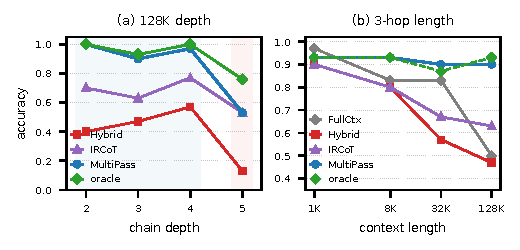
\includegraphics[width=\linewidth]{dkmp_summary_singlecol.pdf}
\caption{Audited DKMP results used in the main text. (a) At $N{=}128$K,
\ours{} repairs 2/3/4-hop bridge starvation and approaches the
gold-support oracle; 5-hop is a boundary case. (b) On 3-hop chains, the
failure is context-length conditional: single-pass Hybrid-RRF and FullCtx
degrade as context grows, while \ours{} remains close to oracle through
128K.}
\label{fig:dkmp-summary}
\end{figure}

\begin{table*}[t]
\centering
\caption{Multi-hop accuracy at $N{=}128$K, GLM-4.7 LLM-judged
($n{=}30$/cell). Bootstrap 95\% CIs in brackets (10K resamples) for the
three methods most discussed in the text. \ours{} matches oracle on 2-hop
and is within 3pp of oracle on 3/4-hop. At 5-hop, \ours{} no longer wins
(\Cref{sec:saturation}).}
\label{tab:main}
\small
\begin{tabular}{@{}lcccc@{}}
\toprule
Method & 2-hop & 3-hop & 4-hop & 5-hop \\
\midrule
FullCtx (8K trunc) & 0.87 [0.73,0.97] & 0.50 [0.33,0.67] & 0.83 [0.70,0.97] & 0.80 [0.63,0.93] \\
BM25 top-10 & 0.33 & 0.33 & 0.50 & 0.20 \\
Hybrid-RRF top-10 & 0.40 & 0.47 & 0.57 & 0.13 \\
PPR (HippoRAG-style) & 0.07 & 0.13 & 0.40 & 0.03 \\
IRCoT 0-shot & 0.87 & 0.60 & 0.77 & 0.84 \\
IRCoT 8-shot faithful & 0.70 [0.53,0.87] & 0.63 [0.47,0.80] & 0.77 [0.60,0.90] & 0.53 [0.37,0.70] \\
ReAct & 0.60 & 0.53 & 0.53 & 0.60 \\
Self-Ask & 0.30 & 0.33 & 0.30 & 0.37 \\
\textbf{\ours{} (ours)} & \textbf{1.00 [1.00,1.00]} & \textbf{0.90 [0.80,1.00]} & \textbf{0.97 [0.90,1.00]} & 0.53 [0.37,0.70] \\
\midrule
Oracle (gold needles) & 1.00 & 0.93 & 1.00 & 0.76 \\
\bottomrule
\end{tabular}
\end{table*}

The targeted regime is 2/3/4-hop reasoning at $N{=}128$K
(\Cref{fig:dkmp-summary}a). In this regime, \ours{} is within 3pp of
oracle on every depth. Compared with IRCoT 8-shot
faithful, the gap is +30pp on 2-hop, +27pp on 3-hop, and +20pp on 4-hop.
The corresponding gaps over ReAct are +37 / +37 / +44pp, and the gaps over
Self-Ask are +70 / +57 / +67pp. The confidence intervals do not overlap on
2-hop and touch only at the endpoint on 3-hop.

A natural concern is that 0-shot IRCoT may understate the original method
by omitting demonstrations. We therefore include an 8-shot faithful IRCoT
variant with eight hand-crafted DKMP-style demonstrations,
\texttt{remove\_wh\_words}, reasoning-sentence skip for next-query
selection, and \texttt{max\_steps=8}. Both IRCoT variants lose to \ours{}
on 2/3/4-hop by 20--30pp. The 8-shot variant is worse than 0-shot on
2-hop and 5-hop, likely because the demonstrations bias the model toward
their chain structure even when the synthetic entities differ.

\subsection{Length Curve: the Trigger is Context-Length Conditional}\label{sec:lengths}

\begin{table}[t]
\centering
\caption{3-hop accuracy across context lengths. The single-pass failure
emerges in the 8K--32K band; \ours{} is the only method that holds at
$N{=}128$K.}
\label{tab:lengths}
\small
\begin{tabular}{@{}lcccc@{}}
\toprule
Method & N=1K & N=8K & N=32K & N=128K \\
\midrule
FullCtx & 0.97 & 0.83 & 0.83 & 0.50 \\
Hybrid-RRF & 0.90 & 0.80 & 0.57 & 0.47 \\
IRCoT 8-shot & 0.90 & 0.80 & 0.67 & 0.63 \\
ReAct & 0.60 & 0.63 & 0.37 & 0.53 \\
\textbf{\ours{}} & \textbf{0.93} & \textbf{0.93} & \textbf{0.90} & \textbf{0.90} \\
Oracle & 0.93 & 0.93 & 0.87 & 0.93 \\
\bottomrule
\end{tabular}
\end{table}

\Cref{fig:dkmp-summary}b and \Cref{tab:lengths} show that the failure is
not a generic multi-hop deficit. At 1K, FullCtx, Hybrid-RRF, IRCoT, and
\ours{} all score at least 0.90 on 3-hop chains except ReAct. The gap opens
as the context grows: Hybrid-RRF drops to 0.57 at 32K and 0.47 at 128K,
while \ours{} stays at 0.90. This pattern supports the trigger definition
in \Cref{sec:dkmp}: bridge starvation requires both a multi-hop chain and
a context long enough that simply reading everything is unreliable.

\section{Cost and Repair Budget}\label{sec:cost}

\begin{figure}[t]
\centering
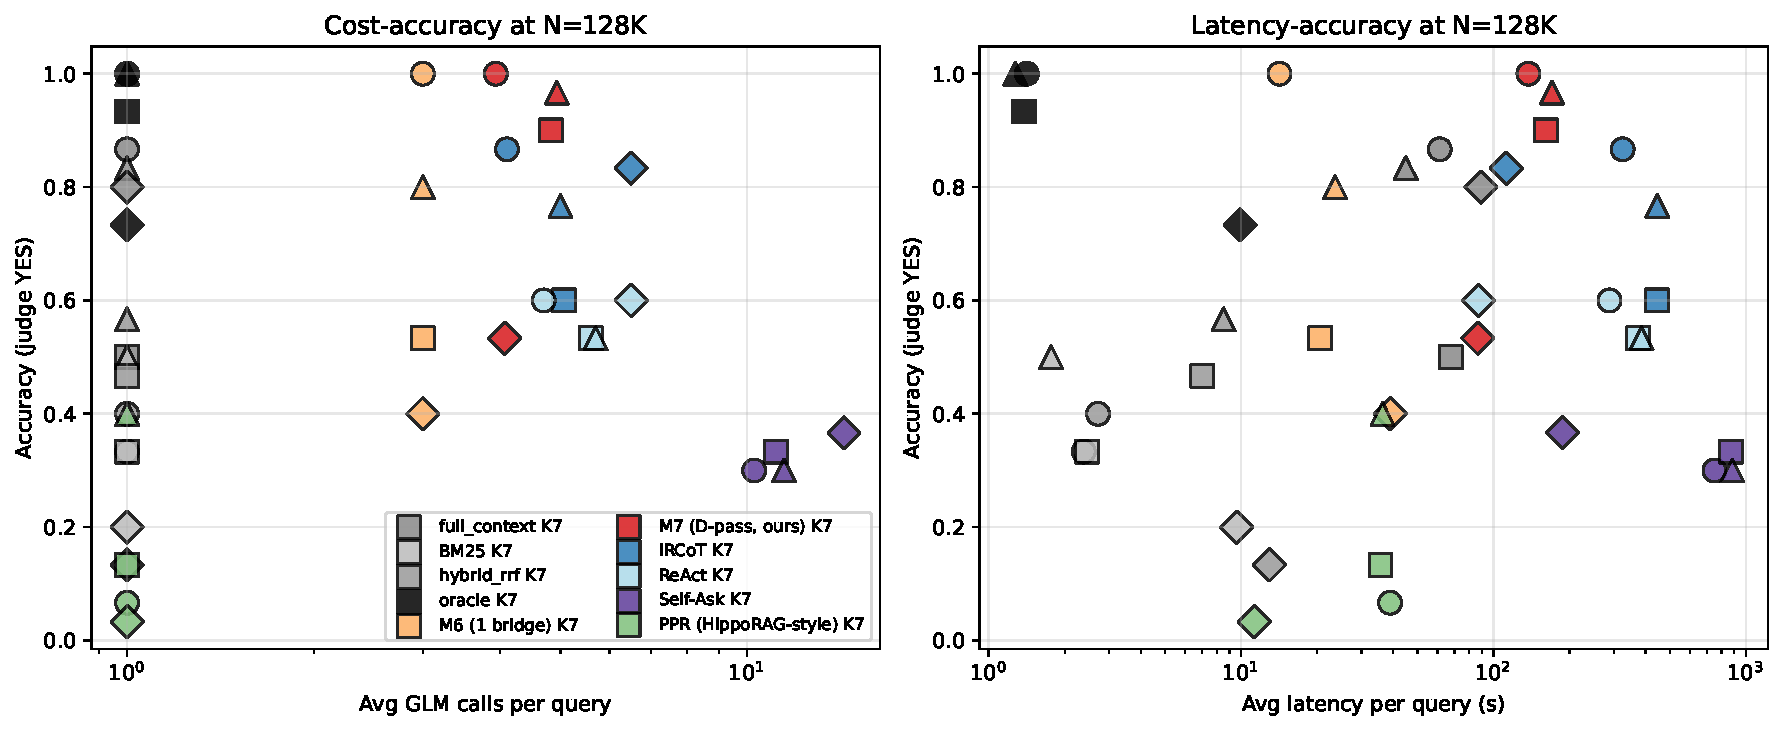
\includegraphics[width=\linewidth]{cost_pareto.pdf}
\caption{Cost--accuracy points on multi-hop chains at $N{=}128$K. Each
marker is a $(\text{method}, D)$ cell. Among iterative-retrieval methods,
\ours{} is upper-left on both axes. FullCtx has fewer LLM calls and lower
latency but uses ${\sim}22\times$ more reader tokens and is less accurate
in the targeted regime.}
\label{fig:pareto}
\end{figure}

\begin{table}[t]
\centering
\caption{Per-query cost on 2/3/4-hop at $N{=}128$K (averaged over 90
queries). \ours{} is the cheapest among iterative-retrieval methods on
both LLM calls and end-to-end latency, and the highest-accuracy method
overall except oracle. FullCtx has lower latency than \ours{} but uses
${\sim}22\times$ more reader tokens.}
\label{tab:cost}
\small
\begin{tabular}{@{}lrrrr@{}}
\toprule
Method & Calls & Tokens & Lat.~(s) & Acc \\
\midrule
FullCtx & 1.0 & 128{,}007 & 65.8 & 0.73 \\
Hybrid-RRF & 1.0 & 2{,}044 & 7.8 & 0.48 \\
PPR & 1.0 & 5{,}600 & 37.0 & 0.20 \\
\textbf{\ours{}} & \textbf{4.6} & 5{,}650 & \textbf{156} & \textbf{0.96} \\
IRCoT 8-shot & 5.5 & 6{,}500 & 470 & 0.70 \\
ReAct & 5.3 & 2{,}378 & 350 & 0.55 \\
Self-Ask & 11.0 & 2{,}689 & 836 & 0.31 \\
\midrule
Oracle (gold) & 1.0 & 41 & 3.6 & 0.98 \\
\bottomrule
\end{tabular}
\end{table}

The latency gap between \ours{} (156s) and IRCoT 8-shot (470s) is
${\approx}3\times$. The gap arises because \ours{}'s bridge call output is
capped at 30 tokens while IRCoT emits a full CoT sentence per step;
asynchronous queueing under load amplifies the per-step difference.
Self-Ask is the most expensive because it issues both a decomposition call
\emph{and} a sub-question answer call per follow-up. We report calls,
tokens, and latency; we do not convert to dollar cost because the
provider's token rates may change.

% =============================================================================
\section{Boundary and Negative Results}\label{sec:boundary}

\subsection{5-hop: a boundary, not a tuned success}\label{sec:saturation}

\ours{} 5-hop accuracy is 0.53 [0.37, 0.70], tied with IRCoT 8-shot and
below FullCtx (0.80) and IRCoT 0-shot (0.84). \ours{} does not solve 5-hop.

\Cref{tab:coverage} shows that on 5-hop \ours{} reaches full chain
coverage on only 12 of 30 cases (40\%), versus 27--30 of 30 on 2/3/4-hop.
Of the 12 full-coverage cases, the reader is correct on 11 (0.92); of the
18 partial-coverage cases, only 5 are correct (0.28). The aggregate
gold-support oracle accuracy of 0.76 also shows that 5-step composition is
difficult even when the support is provided directly.

The 5-hop boundary therefore has two causes. The larger one in our setup
is retrieval: the bridge LLM is accurate (0.98 hit rate, \Cref{tab:bridge}),
but a correctly named bridge entity can recur in distractor passages and
fill the top-$K$ window with non-gold matches. The second cause is reader
composition: even with gold support, 5-step reasoning is near the reader's
ability boundary. \ours{} targets bridge starvation, not these two later
failure modes.

\subsection{Short context: the trigger does not fire}\label{sec:musique}

\begin{table}[t]
\centering
\caption{MuSiQue val ($n{=}300$ balanced 2/3/4-hop, GLM-4.7 LLM-judged).
Each MuSiQue question has 20 short paragraphs, total context ${\sim}5K$
characters. Below the trigger preconditions in \Cref{sec:dkmp};
single-pass retrieval, FullCtx, and \ours{} cluster around 0.49.}
\label{tab:musique}
\small
\begin{tabular}{@{}lcccc@{}}
\toprule
Method & All & 2-hop & 3-hop & 4-hop \\
\midrule
\ours{} & 0.490 & 0.550 & 0.560 & 0.360 \\
ReAct & 0.493 & 0.460 & 0.550 & 0.470 \\
FullCtx & 0.493 & 0.530 & 0.520 & 0.430 \\
IRCoT & 0.473 & 0.580 & 0.500 & 0.340 \\
Hybrid-RRF & 0.387 & 0.440 & 0.450 & 0.270 \\
Self-Ask & 0.223 & 0.400 & 0.170 & 0.100 \\
Oracle (supporting) & 0.753 & 0.760 & 0.770 & 0.730 \\
\bottomrule
\end{tabular}
\end{table}

The MuSiQue tie is non-trigger evidence: \dkmp{}'s length curve places
the trigger boundary in the 8K--32K range. MuSiQue at 5K is below it,
so single-pass retrieval and FullCtx work and \ours{} has nothing to
repair. We do not claim improvement where the failure does not exist.

\subsection{LongMemEval: same-reader fairness check}\label{sec:longmemeval}

\lm{}'s dominant failure type is cross-session aggregation (e.g., ``How
many model kits have I bought?''), not chain traversal. \ours{}'s bridge
mechanism does not help because there is no obvious next-entity to
retrieve. We include \lm{} as a same-reader fairness check on
agentic-memory baselines.

\begin{table*}[t]
\centering
\caption{\lm{} N=500, GLM-4.7 LLM-judged. This is a same-reader fairness
check, not a claim against the published Mem0 or A-Mem systems. Under the
fixed reader used here, chunk retrieval over raw conversation transcripts
is strongest overall; Mem0-style wins KU and Temp but loses SA/SU, showing
that memory representation and reader choice must be separated.}
\label{tab:longmemeval}
\small
\begin{tabular*}{\textwidth}{@{\extracolsep{\fill}}lcccccc@{}}
\toprule
Method & Overall & KU & MS & Temp & SA & SU \\
\midrule
FullCtx (8K trunc) & 0.360 & 0.128 & 0.120 & 0.195 & 0.982 & 0.814 \\
Oracle (gold sessions) & 0.384 & 0.141 & 0.105 & 0.203 & 0.982 & 0.957 \\
BM25 chunks K=10 & 0.612 & 0.692 & 0.481 & 0.398 & 0.982 & 0.929 \\
Dense chunks K=10 & 0.608 & 0.603 & 0.579 & 0.316 & 0.982 & 0.929 \\
\textbf{Hybrid-RRF K=10} & \textbf{0.614} & 0.667 & 0.526 & 0.361 & 0.982 & 0.943 \\
Mem0-style & 0.562 & 0.718 & 0.481 & 0.541 & 0.464 & 0.714 \\
A-Mem-style & 0.520 & 0.603 & 0.436 & 0.474 & 0.482 & 0.657 \\
\bottomrule
\end{tabular*}
\end{table*}

Mem0-style wins on KU and Temp (where extraction filters chitchat) but
loses on SA/SU (where the reader needs the original surface form).
Aggregate Hybrid-RRF wins by 5.2pp. Read this as a fairness reminder:
published agentic-memory numbers often change both the memory
representation and the reader; same-reader comparisons are needed to
isolate the memory-side contribution.

\subsection{Cross-reader check}\label{sec:crossreader}

\begin{table}[t]
\centering
\caption{Cross-reader: \ours{} at $N{=}128$K with GLM-4.7 vs.\
GPT-4o-mini ($n{=}30$). Single-pass Hybrid-RRF (GLM-4.7) shown for
reference. The repair transfers across the two readers we tested.}
\label{tab:crossreader}
\small
\begin{tabular}{@{}lccc@{}}
\toprule
Hop & GLM & GPT & Hybrid \\
\midrule
2-hop & 1.00 & 0.97 & 0.40 \\
3-hop & 0.90 & 0.80 & 0.47 \\
4-hop & 0.97 & 0.90 & 0.57 \\
\bottomrule
\end{tabular}
\end{table}

% =============================================================================
\section{Limitations}\label{sec:limits}

The main DKMP cells have $n{=}30$, so several confidence intervals remain
wide; the paper should be read as a reproducible trigger and diagnostic
study, not as a final leaderboard. We test GLM-4.7 fully and GPT-4o-mini on
the cross-reader slice, but not Claude- or Llama-class readers. The trigger
uses synthetic-entity needles embedded in real fictional contexts; this
prevents world-knowledge shortcuts, but it does not replace a natural
long-context multi-hop benchmark. Finally, the HippoRAG-style PPR baseline
uses chunk-cosine edges rather than a fully faithful OpenIE graph, and our
IRCoT 8-shot demonstrations are DKMP-style rather than unchanged HotpotQA
prompts because the synthetic entity vocabulary is incompatible.
We use a separate LLM call for judging, but the judge is still an automatic
judge from the same model family as the reader; a human-audited subset
would make the error analysis stronger.

% =============================================================================
\section{Conclusion}\label{sec:conclusion}

We isolated and operationalized one failure of single-pass agentic-memory
retrieval at long context: bridge starvation. \dkmp{} reproduces the
failure under a fixed protocol and exposes the missing links in the trace.
\ours{} is a minimal repair; it works in the targeted regime, has measured
cost, and has explicit boundaries where it does not work. We hope the
trigger and the trace diagnostic are reusable.

\bibliographystyle{icml2026}
\bibliography{paper}

\appendix

\section{Concrete trace example}\label{appx:trace}

A real DKMP 3-hop instance from our logs.

\medskip
\textbf{Story:} \texttt{dkmp\_1b82b150} (NarrativeQA-derived distractor,
$N{=}128$K).

\textbf{Chain:} ``Hartin Whatley purchased the Sapphire of Telemar.'' $\to$
``The Sapphire of Telemar was originally cut in the city of Bryandyl.''
$\to$ ``Bryandyl is renowned for saffron-laced cordials.''

\textbf{Question:} ``What is the most famous export of the city where
Hartin Whatley's purchase was originally cut?''

\textbf{Single-pass top-10 hybrid retrieval:} returns the Hartin Whatley
needle and 9 distractor chunks; \emph{misses} both Bryandyl needles.
Reader: ``unknown / unspecified.''

\textbf{\ours{}:}
\begin{itemize}\setlength{\itemsep}{0.02em}
  \item Pass 1: same retrieval as single-pass.
  \item Bridge LLM, given Hartin's needle: ``Sapphire of Telemar.''
  \item Pass 2: retrieves the Bryandyl-cutting needle.
  \item Bridge LLM: ``Bryandyl.''
  \item Pass 3: retrieves the Bryandyl-cordials needle.
  \item Bridge LLM: ``NONE.''
  \item Reader: ``saffron-laced cordials.'' Judge: YES.
\end{itemize}

\section{Ablations}\label{appx:ablation}

All on 3-hop chains, $N{=}128$K, $n{=}30$, lenient string match (faster
than the GLM judge for sweeps; trends are robust to switching to the GLM
judge on a 30-row spot check).

\begin{itemize}\setlength{\itemsep}{0.05em}
  \item \ours{} max-passes sweep: 1 / 2 / 3 / 4 / 5 / 6 / 7
        $\to$ 0.43 / 0.50 / 0.93 / 0.90 / 0.87 / 0.83 / 0.90.
        Match-or-exceed-chain-depth is necessary; beyond that, the
        LLM-NONE early-stop kicks in and accuracy plateaus.
  \item Bridge-prompt length cap (words): 3 / 6 / 12 / 25
        $\to$ 0.73 / 0.70 / 0.77 / 0.67. Caps from 3 to 12 are within
        noise; the 25-word ``full sentence'' variant degrades.
  \item Top-$K$ per pass: 3 / 5 / 10 / 20
        $\to$ 0.67 / 0.63 / 0.73 / 0.77. Diminishing returns appear above
        $K{=}10$.
\end{itemize}

\section{Reproducibility}\label{appx:repro}

\begin{itemize}\setlength{\itemsep}{0.05em}
  \item All code, prompts, seeds, and per-cell predictions released
        alongside the paper (see supplementary).
  \item Total compute: ${\sim}12$ hours wall-time on a single laptop
        (M-series MPS for BGE-M3 chunk embeddings).
  \item Each method uses the same retrieval index (BGE-M3 + BM25 fused
        via reciprocal rank fusion) and the same reader prompt; the
        only difference is the bridge or reasoning loop.
  \item All judges use a fresh GLM-4.7 instance with a YES/NO prompt
        disjoint from the reader prompt.
  \item Bootstrap CIs use 10K resamples with seed 42.
\end{itemize}

\end{document}
